\documentclass{article}

% Just to have them already
% \begin{sloppypar}
% \end{sloppypar}


% Just try to parse, do not ask for input
\nonstopmode

% Bibliography
\usepackage{natbib}
\bibpunct{(}{)}{;}{a}{}{;}

% Use 'It was found that A is B (Name 1234)' style
\setcitestyle{authoryear,open={},close={}}

% Affiliations
\usepackage{authblk}
\title{
  Transmembrane helices are also 
  an overlooked source of major histocompatibility complex class II epitopes
  and evolutionary more conserved than expected by chance
}
\author[1]{Richèl J.C. Bilderbeek}
\author[1]{Maxim Baranov}
\author[1]{Geert van den Bogaart}
\author[1]{Frans Bianchi}
\affil[1]{GBB, University of 
Groningen, Groningen, The Netherlands}

% Use double spacing
\usepackage{setspace}
\doublespacing

\usepackage{listings}
\usepackage{hyperref}
\usepackage{todonotes}
\usepackage{verbatim}
\usepackage{pgf}
\usepackage{bm}
\usepackage{multirow}
\usepackage{amsfonts}
\usepackage{array}
\usepackage{booktabs}
\newcolumntype{C}[1]{>{\centering\arraybackslash}p{#1}}
\newcolumntype{L}[1]{>{\raggedright\arraybackslash}p{#1}}
\usepackage{longtable}

\usepackage{tkz-graph}
\usetikzlibrary{arrows,automata}
\usetikzlibrary{calc}
\usetikzlibrary{arrows.meta}

% sidewaysfigure
\usepackage{rotating}

% Style of listings
% From http://r.789695.n4.nabble.com/
%   How-to-nicely-display-R-code-with-the-LaTeX-package-listings-tp4648110.html
\usepackage{fancyvrb} 
\definecolor{codegreen}{rgb}{0,0.6,0}
\definecolor{codegray}{rgb}{0.5,0.5,0.5}
\definecolor{codepurple}{rgb}{0.58,0,0.82}
\definecolor{backcolor}{rgb}{0.95,0.95,0.92}
\lstdefinestyle{mystyle}{
  language=R,% set programming language
  basicstyle=\ttfamily\small,% basic font style
  commentstyle=\color{gray},% comment style
  numberstyle=\scriptsize,% use small line numbers
  numbersep=10pt,% space between line numbers and code
  tabsize=2,% sizes of tabs
  showstringspaces=false,
  captionpos=b,% positioning of the caption below
  breaklines=true,% automatic line breaking
  escapeinside={(*}{*)},% escaping to LaTeX
  fancyvrb=true,% verbatim code is typset by listings
  extendedchars=false,% prohibit extended chars (chars of codes 128--255)
  alsoletter={.<-},% becomes a letter
  alsoother={$},% becomes other
  otherkeywords={!=, ~, $, \&, \%/\%, \%*\%, \%\%, <-, <<-, /},
  deletekeywords={c}% remove keywords 
}
\lstset{style=mystyle}

% Adds numbered lines. Not yet...
% \usepackage{lineno}
% \linenumbers

%comments
\newcommand{\frans}[1]{\textcolor{blue}{\textbf{[FB: #1]}}}
\newcommand{\richel}[1]{\textcolor{orange}{\textbf{[RB: #1]}}}

\begin{document}

\maketitle

\begin{abstract}

Transmembrane helices (TMHs) in the human proteome
are an overrepresented potential source of epitopes on major 
histocompatibility complex (MHC) class I for the majority of HLA-I haplotypes. 
It is unknown if the immune system is as able to detect those 
TMHs present in pathogens.
Additionally, it is unknown if TMH-II is also likelier to detect
human and pathogen TMHs than expected by chance.
It is unknown if natural selection is the cause that 
the immune system is more attentive for TMHs
This study shows that MHC-I [also has/does not have] more
epitopes derived from a TMH for a pathogen proteome, when compared with
a host proteome.
Additionally, MHC-II binds to polypeptides derived from TMHs 
[less/equally/more] often than expected by chance.
Lastly, we show that natural selection on TMHs is [strong enough/still too weak]
to detect.
Our findings suggest that the immune system is [less/neutral/more]
vigilant to TMHs than expected by chance and this has 
left [a clear/a weak/no]
signal in the evolutionary history of the pathogen.

\end{abstract}

{\bf Keywords:} antigen presentation, membrane proteins, bioinformatics, 
adaptive immunity, transmembrane domain, epitopes, T lymphocyte, 
MHC-1, MHC-I, MHC-2, MHC-II, COVID-19

%%%%%%%%%%%%%%%%%%%%%%%%%%%%%%%%%%%%%%%%%%%%%%%%%%%%%%%%%%%%%%%%%%%%%%%%%%%%%%%%
\section{Introduction}
%%%%%%%%%%%%%%%%%%%%%%%%%%%%%%%%%%%%%%%%%%%%%%%%%%%%%%%%%%%%%%%%%%%%%%%%%%%%%%%%

\paragraph{Immune response}

\richel{Check for correctness}
Our immune system fights invaders on a daily basis.
These invaders can be fungi, bacteria or viruses.
The innate immune response is its first general 
and immediate strategy, where the acquired immune response
needs time to develop its specialized and more effective
combat forces.

\paragraph{Immune response by MHC-I}

\richel{Check for correctness}
All nucleated cells in humans present randomly sampled polypeptides
fragments to the surroundings of the cell using MHC class I molecules.
If a cell gets infected by a virus, also the virus' polypeptides
will be presented at the cell surface. The viral antigen is detected 
by cytotoxic T lymphocytes, which will kill the infected cell.

\paragraph{Immune response by MHC-II}

\richel{Check for correctness}
Bacteria and fungi do not infect a cell with their foreign DNA,
but are detected by the proteins on their cell walls. MHC class II molecules 
bind to specific polypeptide fragments. This binding allows T and B cells,
which all express MHC-II, to detect a pathogen and trigger the response to
kill the pathogen. Note that the foreign proteins of a viral envelope 
can be detected in this way as well, which is commonly used in vaccination.

\paragraph{MHCs bind hydrophobic epitopes}

\richel{Check for correctness}
Any human's immune system detects only a fraction of all possible
polypeptide fragments. 
Already each MHC molecule can only bind a
subset of all possible polypeptides. 
The polypeptides that can bind are also likelier to by hydrophobic,
as most TMHs have a hydrophobic binding pocket \richel{Reference needed}.
There are two sources of hydrophobic polypeptides, which are 
from membrane proteins and of soluble proteins.
Membrane proteins have at least one TMH to anchor them to
the membrane. TMHs are hydrophobic, as this is required to span the 
hydrophobic cellular lipid membrane. Additionally,
they often have a length of 23 amino acids to be able to span
the membrane.
Soluble proteins have (non-TMH) hydrophobic regions as well, 
to guides the protein to achieve its 3D configuration.

\paragraph{MHC-I presents hydrophobic regions more often}

One might expect that the hydrophobic epitopes presented,
for a same hydrophobicity, are as likely to stem from 
membrane proteins TMHs or from soluble proteins hydrophobic (non-TMH) regions.
For MHC-I, however, it is found that the 9-mers stemming
from TMHs are presented more often than expected by 
chance \cite{bianchi2017}
\richel{but also when compensating for hydrophobicity?}.
For MHC-II, it is unknown which percentage of binders 
is derived from TMHs for all 13-mers present in a proteome
that have the same hydrophobicity 
\richel{
  $\mathcal{H}_{3,1}$
}.

\paragraph{HLAs increase detection range}

An increased detection
is obtained by expressing a wide variety of
MHCs, which is assured by the human leukocyte antigen gene complex (HLA).
However, a different HLA will result in a different variety of MHCs,
that will display different polypeptide fragments. Additionally, there
may have been selection the HLA to display and or detect different
polypeptide fragments.

\paragraph{MHC-I presents TMH-derived epitopes in humans more often}

\richel{Check for correctness}
For MHC-I, it was found that predicted epitopes derived 
from human transmembrane helices (TMHs)
are over-presented by all HLA-A and 
most HLA-B super types (\cite{bianchi2017}). 
One explanation is that the presentation of TMHs 
may have an evolutionary advantage for 
the (human) host, as TMHs have a reduced variability 
due to the functional requirement of being able to span a lipid 
bilayer. 
Due to this, pathogens have a lower chance to develop an escape mutation,
as many mutations will result in a disfunctional TMH.
Note that the mechanism by which a cell presents its TMHs is
yet unknown.

\paragraph{Does MHC-I present TMH-derived epitopes from pathogens as often?}

It is important that MHC-I presents both the polypeptides of the 
(healthy) cell, as well as possible pathogen-derived polypeptides when the
cell is infected. As described above, MHC-I presents TMH-derived epitopes 
from the human host more often. It is unknown if MHC-I has the same
dedication to present epitopes that stem from TMHs derived from
proteins produced by pathogen, either would the pathogen
be a virus \richel{$\mathcal{H}_{1,1}$} or 
a bacterium \richel{$\mathcal{H}_{1,2}$}.


\paragraph{MHC-II is expected to present TMHs}

\richel{Check for correctness}
If presentation of TMHs on MHC-I would bring an evolutionary advantage 
in the recognition of pathogens by the immune system, 
it would follow that this is equally important for MHC-II, 
especially as the help of CD4+ T cells is needed for a long lasting CD8+ T cell 
response \cite{novy2007cd4}. 
The mechanism to detect foreign TMHs by MHC-II would be unknown, 
similar to the discovery that MHC-I presents TMHs.

\paragraph{Does MHC-II present TMH-derived epitopes from pathogens as often?}

It is unknown if MHC-II, like MHC-I, 
present TMH-derived epitopes as as often, either 
in humans \richel{$\mathcal{H}_{2,1}$},
bacteria \richel{$\mathcal{H}_{2,2}$}
or viruses \richel{$\mathcal{H}_{2,3}$}.

\paragraph{Selection undetectable in whole proteome}

\richel{Check for correctness}
The human immune system and human pathogen are in an evolutionary
arms race: our immune systems is selected for the detection
of pathogens, whereas pathogens are selected to avoid detection.
From a pathogen's point of view, however, this struggle 
is of only minor importance:
in seasonal influenza, for example, the selection pressure
exerted by the immune system was only limited \cite{han2019individual}
\richel{but this study does not look into the evolution of TMHs}.
In general, on would expect that evolutionary selection is strongest 
for regions that are important for viral proteins' functions:
in COVID-19, for example, there is preliminary evidence that the strongest
selection pressure is upon residues that changes its virulence \cite{velazquez2020positive}
\richel{residue 251 of ORF3a (an ion channel and a 
viroporin, residue is not part of TMH), and position 84 of ORF8 (unknown function)}.
The part of a pathogen's proteome that is essential, 
only accounts for small part of its full proteome.
Also, these essential parts differ widely between pathogens.
Because of this scarcity and variance in targets, 
one expects that the human immune system
is not tailored to detect these sites, 
as hinted by upon by the aforementioned influenza study.

\paragraph{Selection may be detectable in TMHs}

TMHs, on the other hand, also have their function constraints, 
yet can occur multiple time a pathogen's proteome.
One can safely assume a pathogen's proteome contains multiple TMHs.
Therefore, it may be beneficial for the host
if its immune system would be more attentive towards TMHs.
And maybe this has already happened: MHC-I already detects hydrophobic
polypeptides. This feature, however, may also be caused by selection
to detect hydrophobic regions in the soluble proteins of pathogens.
It is unknown, when focusing on TMHs only, if a signal of selection
can be detected.

\paragraph{Use of protein data in phylogenetics}

When using DNA sequences, one can use $dS/dN$ rates 
to detect the signature of selection \cite{murrell2015gene}.
Using AA sequences, however, has its advantages,
as its is closer to the actual phenotype
selection acts upon: DNA may never be translated to RNA,
or its RNA may never be transcribed \cite{diz2012proteomics}
\richel{improve upon this point}.
When using a proteome in phylogenetic research,
we know that the majority of proteins are selected to just 
maintain their function most of the time, where
is the time spans there is selection, only a few AAs
can actually increase the 'fitness' of the 
protein \cite{anisimova2009investigating}.
There, when generalizing the dynamics of mostly purifying selection (to maintain
a protein's function) and a short duration of positive selection,
those genes that are selected cannot be detected \cite{yang2000statistical}.

\paragraph{Evolutionary signal of unknown strength for virus}

\richel{Check for correctness}
Regarding human viruses, we do not know the selection pressure
exerted by the human immune system.
For viral TMHs that are undetected by most human haplotypes, we
expect these to be conserved, to remain avoiding detection.
For viral TMHs that are detected by most human haplotypes, we
expect there to be a higher mutation rate, to avoid detection.
Additionally, viruses are not only selected for their evasion of an 
immune response, yet are selected to have a high reproductive value.
Because the strength of the evolutionary signal is unknown,
we use a strong data set to be able to detect it.

\paragraph{Evolutionary signal of unknown strength for bacteria}

\richel{Check for correctness}
Regarding human pathogenic bacteria, we do not know the extent to which the 
human immune systems selects on these, nor which loci are selected
upon \richel{so I should read the literature on that}.
Because most bacterial pathogens are generalists, that is,
can infect multiple hosts, we expect the selection pressure exerted
by the human immune response to be weak.
For bacterial TMHs that are undetected by most human haplotypes, we
expect these to be conserved, to remain avoiding detection.
For bacterial TMHs that are detected by most human haplotypes, we
expect there to be a higher mutation rate, to avoid detection.
Also, it is unknown if bacterial TMHs are detected by MHC-II at all.
Due to this, the strength of the evolutionary signal is unknown,
thus we need a strong data set to be able to detect it.

\paragraph{Data sets}

\richel{Check for correctness}
To detect an evolutionary signal for selection on the TMHs of viruses, 
we use the many time-dated COVID-19 proteomes.
We can assume that only after the moment that COVID-19 spilled over 
to humans, it has mostly been the human immune system selecting against
its detection, although this is only part of the selection for 
having a high transmission rate.
To detect an evolutionary signal for selection on the TMHs of bacteria, 
we use the proteomes of Mycobacterium. Mycobacterium is \richel{something}.


%%%%%%%%%%%%%%%%%%%%%%%%%%%%%%%%%%%%%%%%%%%%%%%%%%%%%%%%%%%%%%%%%%%%%%%%%%%%%%%%
\section{Hypotheses}
%%%%%%%%%%%%%%%%%%%%%%%%%%%%%%%%%%%%%%%%%%%%%%%%%%%%%%%%%%%%%%%%%%%%%%%%%%%%%%%%

\richel{Will be moved to supplementary materials}

\begin{itemize}
  \item $\mathcal{H}_{1,1}$: MHC-I has the same percentage of epitopes overlapping
    with TMHs in Homo sapiens as in COVID-19
  \item $\mathcal{H}_{1,2}$: MHC-I has the same percentage of epitopes overlapping
    with TMHs in Homo sapiens as in Mycobacterium
  \item $\mathcal{H}_{2,1}$: MHC-II has the same percentage of epitopes overlapping
    with TMHs as expected by chance in Homo sapiens
  \item $\mathcal{H}_{2,2}$: MHC-II has the same percentage of epitopes overlapping
    with TMHs as expected by chance in COVID-19
  \item $\mathcal{H}_{2,3}$: MHC-II has the same percentage of epitopes overlapping
    with TMHs as expected by chance in Mycobacterium
  \item $\mathcal{H}_{3,1}$: MHC-II haplotypes will display epitopes
    of a certain hydrophobicity, that is as likely to stem from
    a TMH or a non-TMH 13-mer as expected by chance
  \item $\mathcal{H}_{3,2}$: MHC-II haplotypes that have hydrophobic
    binding pockets, will display more epitopes derived from (hydrophobic)
    TMHs
  \item $\mathcal{H}_{3,3}$: MHC-II haplotypes that have binding pockets
    that are only partly hydrophobic, will display more epitopes derived 
    from the flanking regions of TMHs
  \item $\mathcal{H}_{4,1}$: The TMHs of COVID-19
    have the same mutation rate 
    as the cytosolic and extracellular parts of their transmembrane proteins
  \item $\mathcal{H}_{4,2}$: The TMHs of Mycobacterium
    have the same mutation rate 
    as the cytosolic and extracellular parts of their transmembrane proteins
\end{itemize}




%%%%%%%%%%%%%%%%%%%%%%%%%%%%%%%%%%%%%%%%%%%%%%%%%%%%%%%%%%%%%%%%%%%%%%%%%%%%%%%%
\section{Methods}
%%%%%%%%%%%%%%%%%%%%%%%%%%%%%%%%%%%%%%%%%%%%%%%%%%%%%%%%%%%%%%%%%%%%%%%%%%%%%%%%

%%%%%%%%%%%%%%%%%%%%%%%%%%%%%%%%%%%%%%%%%%%%%%%%%%%%%%%%%%%%%%%%%%%%%%%%%%%%%%%%
\subsection{MHC-I}
%%%%%%%%%%%%%%%%%%%%%%%%%%%%%%%%%%%%%%%%%%%%%%%%%%%%%%%%%%%%%%%%%%%%%%%%%%%%%%%%

We used the same analysis as \cite{bianchi2017},
except that instead of a human reference proteome,
we use the proteome of the first sequenced COVID-19 strain (\cite{wu2020new},
GenBank ID of MN908947.3, \url{https://www.ncbi.nlm.nih.gov/nuccore/MN908947})
and a reference Mycobacterium tuberculosis 
proteome (\url{https://www.ebi.ac.uk/reference_proteomes}, UP000001584, 
83332 MYCTU).

Bianchi and colleagues obtained a distribution of 
percentages of MHC-I epitopes overlap with TMHs in Homo sapiens
for the different HLA haplotypes, with an average of 5.3\%.
We obtained a similar distribution of percentages of MHC-I epitopes that 
overlap with TMHs for the different HLA haplotypes, but then applied to
COVID-19 and Mycobacterium.

We compare the distributions of humans and each pathogen
using a two-sample Kolmogorov-Smirnov (KS) test
for a significance level $\alpha = 0.05$.

%%%%%%%%%%%%%%%%%%%%%%%%%%%%%%%%%%%%%%%%%%%%%%%%%%%%%%%%%%%%%%%%%%%%%%%%%%%%%%%%
\subsection{MHC-2}
%%%%%%%%%%%%%%%%%%%%%%%%%%%%%%%%%%%%%%%%%%%%%%%%%%%%%%%%%%%%%%%%%%%%%%%%%%%%%%%%

\richel{Check for correctness}
For MHC-II, we do the same analysis as MHC-I, except for
MHC-II haplotypes. We picked the top 21 MHC-II alleles that are most abundant 
in the current human population (\cite{greenbaum2011functional}).
\frans{Show coverage}
We chose to use 21 alleles to have a similar number of alleles as is done
for MHC-I \richel{Unsure if this was the actual reason}.
Same as \cite{bianchi2017}, we defined the 5\% of polypeptides 
with the lowest IC50 values as binders. We then counted the percentage
of binders that have one or more amino acids that are part of a TMH.


%%%%%%%%%%%%%%%%%%%%%%%%%%%%%%%%%%%%%%%%%%%%%%%%%%%%%%%%%%%%%%%%%%%%%%%%%%%%%%%%
\subsection{Evolutionary conservation}
%%%%%%%%%%%%%%%%%%%%%%%%%%%%%%%%%%%%%%%%%%%%%%%%%%%%%%%%%%%%%%%%%%%%%%%%%%%%%%%%

%%%%%%%%%%%%%%%%%%%%%%%%%%%%%%%%%%%%%%%%%%%%%%%%%%%%%%%%%%%%%%%%%%%%%%%%%%%%%%%%
\subsubsection{Detecting evolution}
%%%%%%%%%%%%%%%%%%%%%%%%%%%%%%%%%%%%%%%%%%%%%%%%%%%%%%%%%%%%%%%%%%%%%%%%%%%%%%%%

	% \frans{
	%   Ik heb zitten denken over de evolutie naast conservering is occurrence ook heel belangrijk. Moeten we de mate van conservering niet wegen ten opzichte van de occurrence.
	%   Wat ik daarmee bedoel is data als je kiest voor een mega geconseveerd epitope maar van dat type komen er maar 40 in een proteome voor versus een minder geconserveerd epitope maar daar zijn wel 100.000 varianten van dan heb je meer kans om 1 van die 100.000 te pakken toch? 
	% }
	% The evolutionary conservation of TMHs was measured from a
	% DNA alignment of multiple transmembrane proteins in multiple
	% species of the mycobacterium bacterial family
	% \richel{how obtained exactly? how alignment done?}
	% \frans{
	% Via entrez en blast 
	%   Ik he been transcript van Maxim ik zal dit proberen te vertalen naar een stukje tekst. 
	% }

%%%%%%%%%%%%%%%%%%%%%%%%%%%%%%%%%%%%%%%%%%%%%%%%%%%%%%%%%%%%%%%%%%%%%%%%%%%%%%%%
\section{Results}
%%%%%%%%%%%%%%%%%%%%%%%%%%%%%%%%%%%%%%%%%%%%%%%%%%%%%%%%%%%%%%%%%%%%%%%%%%%%%%%%

% Poisson binomial distribution

%%%%%%%%%%%%%%%%%%%%%%%%%%%%%%%%%%%%%%%%%%%%%%%%%%%%%%%%%%%%%%%%%%%%%%%%%%%%%%%%
\subsection{MHC-I}
%%%%%%%%%%%%%%%%%%%%%%%%%%%%%%%%%%%%%%%%%%%%%%%%%%%%%%%%%%%%%%%%%%%%%%%%%%%%%%%%

Figure \ref{fig:1} shows the percentages of epitopes overlapping 
with TMHs for a human, COVID-19 and Mycobacterium proteome.
The KS test to determine if these percentages are sampled from
a same distribution resulted in a p-value of \richel{unknown},
which makes us reject/accept the hypothesis that these percentages
are sampled from the same distribution. 

\begin{figure}[!htbp]
  \includegraphics[width=\textwidth]{bbbq_1/fig_bbbq_1_watermarked.png}
  \caption{
    \% epitopes overlapping with transmembrane helix
    for a human, COVID-19 and Mycobacterium proteome.
    \richel{
      the data underlying this figure has been simulated
    }
  }
  \label{fig:1}
\end{figure}

%%%%%%%%%%%%%%%%%%%%%%%%%%%%%%%%%%%%%%%%%%%%%%%%%%%%%%%%%%%%%%%%%%%%%%%%%%%%%%%%
\subsection{MHC-II}
%%%%%%%%%%%%%%%%%%%%%%%%%%%%%%%%%%%%%%%%%%%%%%%%%%%%%%%%%%%%%%%%%%%%%%%%%%%%%%%%

\begin{figure}[!htbp]
  \includegraphics[width=\textwidth]{bbbq_2/fig_bbbq_2_watermarked.png}
  \caption{
    \% epitopes overlapping with transmembrane helix
    for a human, COVID-19 and Mycobacterium proteome.
    \richel{
      the data underlying this figure has been simulated
    }
  }
  \label{fig:2}
\end{figure}

%%%%%%%%%%%%%%%%%%%%%%%%%%%%%%%%%%%%%%%%%%%%%%%%%%%%%%%%%%%%%%%%%%%%%%%%%%%%%%%%
\subsection{Evolutionary conservation}
%%%%%%%%%%%%%%%%%%%%%%%%%%%%%%%%%%%%%%%%%%%%%%%%%%%%%%%%%%%%%%%%%%%%%%%%%%%%%%%%

\begin{figure}[!htbp]
  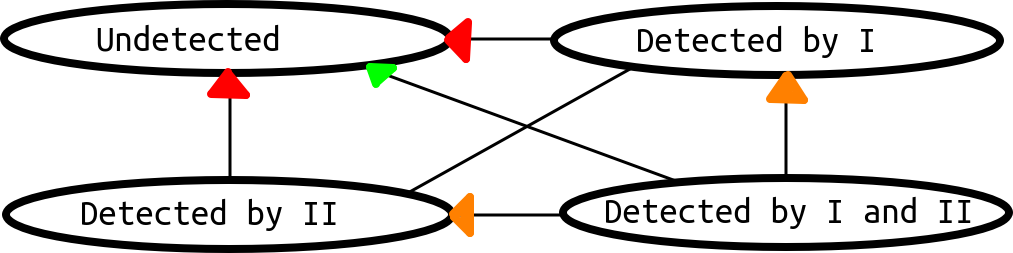
\includegraphics[width=\textwidth]{transitions.png}
  \caption{
    Transitions in TMHs that occur more often then expected by chance,
    for a confidence interval of 5 percent.
    Table \ref{tab:transitions} shows the transition counts.
    \richel{
      stub figure
    }
  }
  \label{fig:transitions}
\end{figure}

\begin{table}[!htbp]
  \input{table_transitions.latex}
  \caption{
    Transitions counts, where the row indicates the source state,
    and the column indicates the target state.
    First number per cell is the observed number of this state transition,
    where the second number is the expected number of this state transition
    as predicted by chance.
    An asterisk behind the observed count indicates that this count
    is unlikely to be caused by chance only.
    Figure \ref{fig:transitions} shows which transition counts are 
    unlikely to be caused by chance only.
  }
  \label{tab:transitions}
\end{table}

	% Table \ref{tab:results} shows the location and binding strength for the
	% tuberculosis proteome.

	% \begin{figure}[ht]
	%   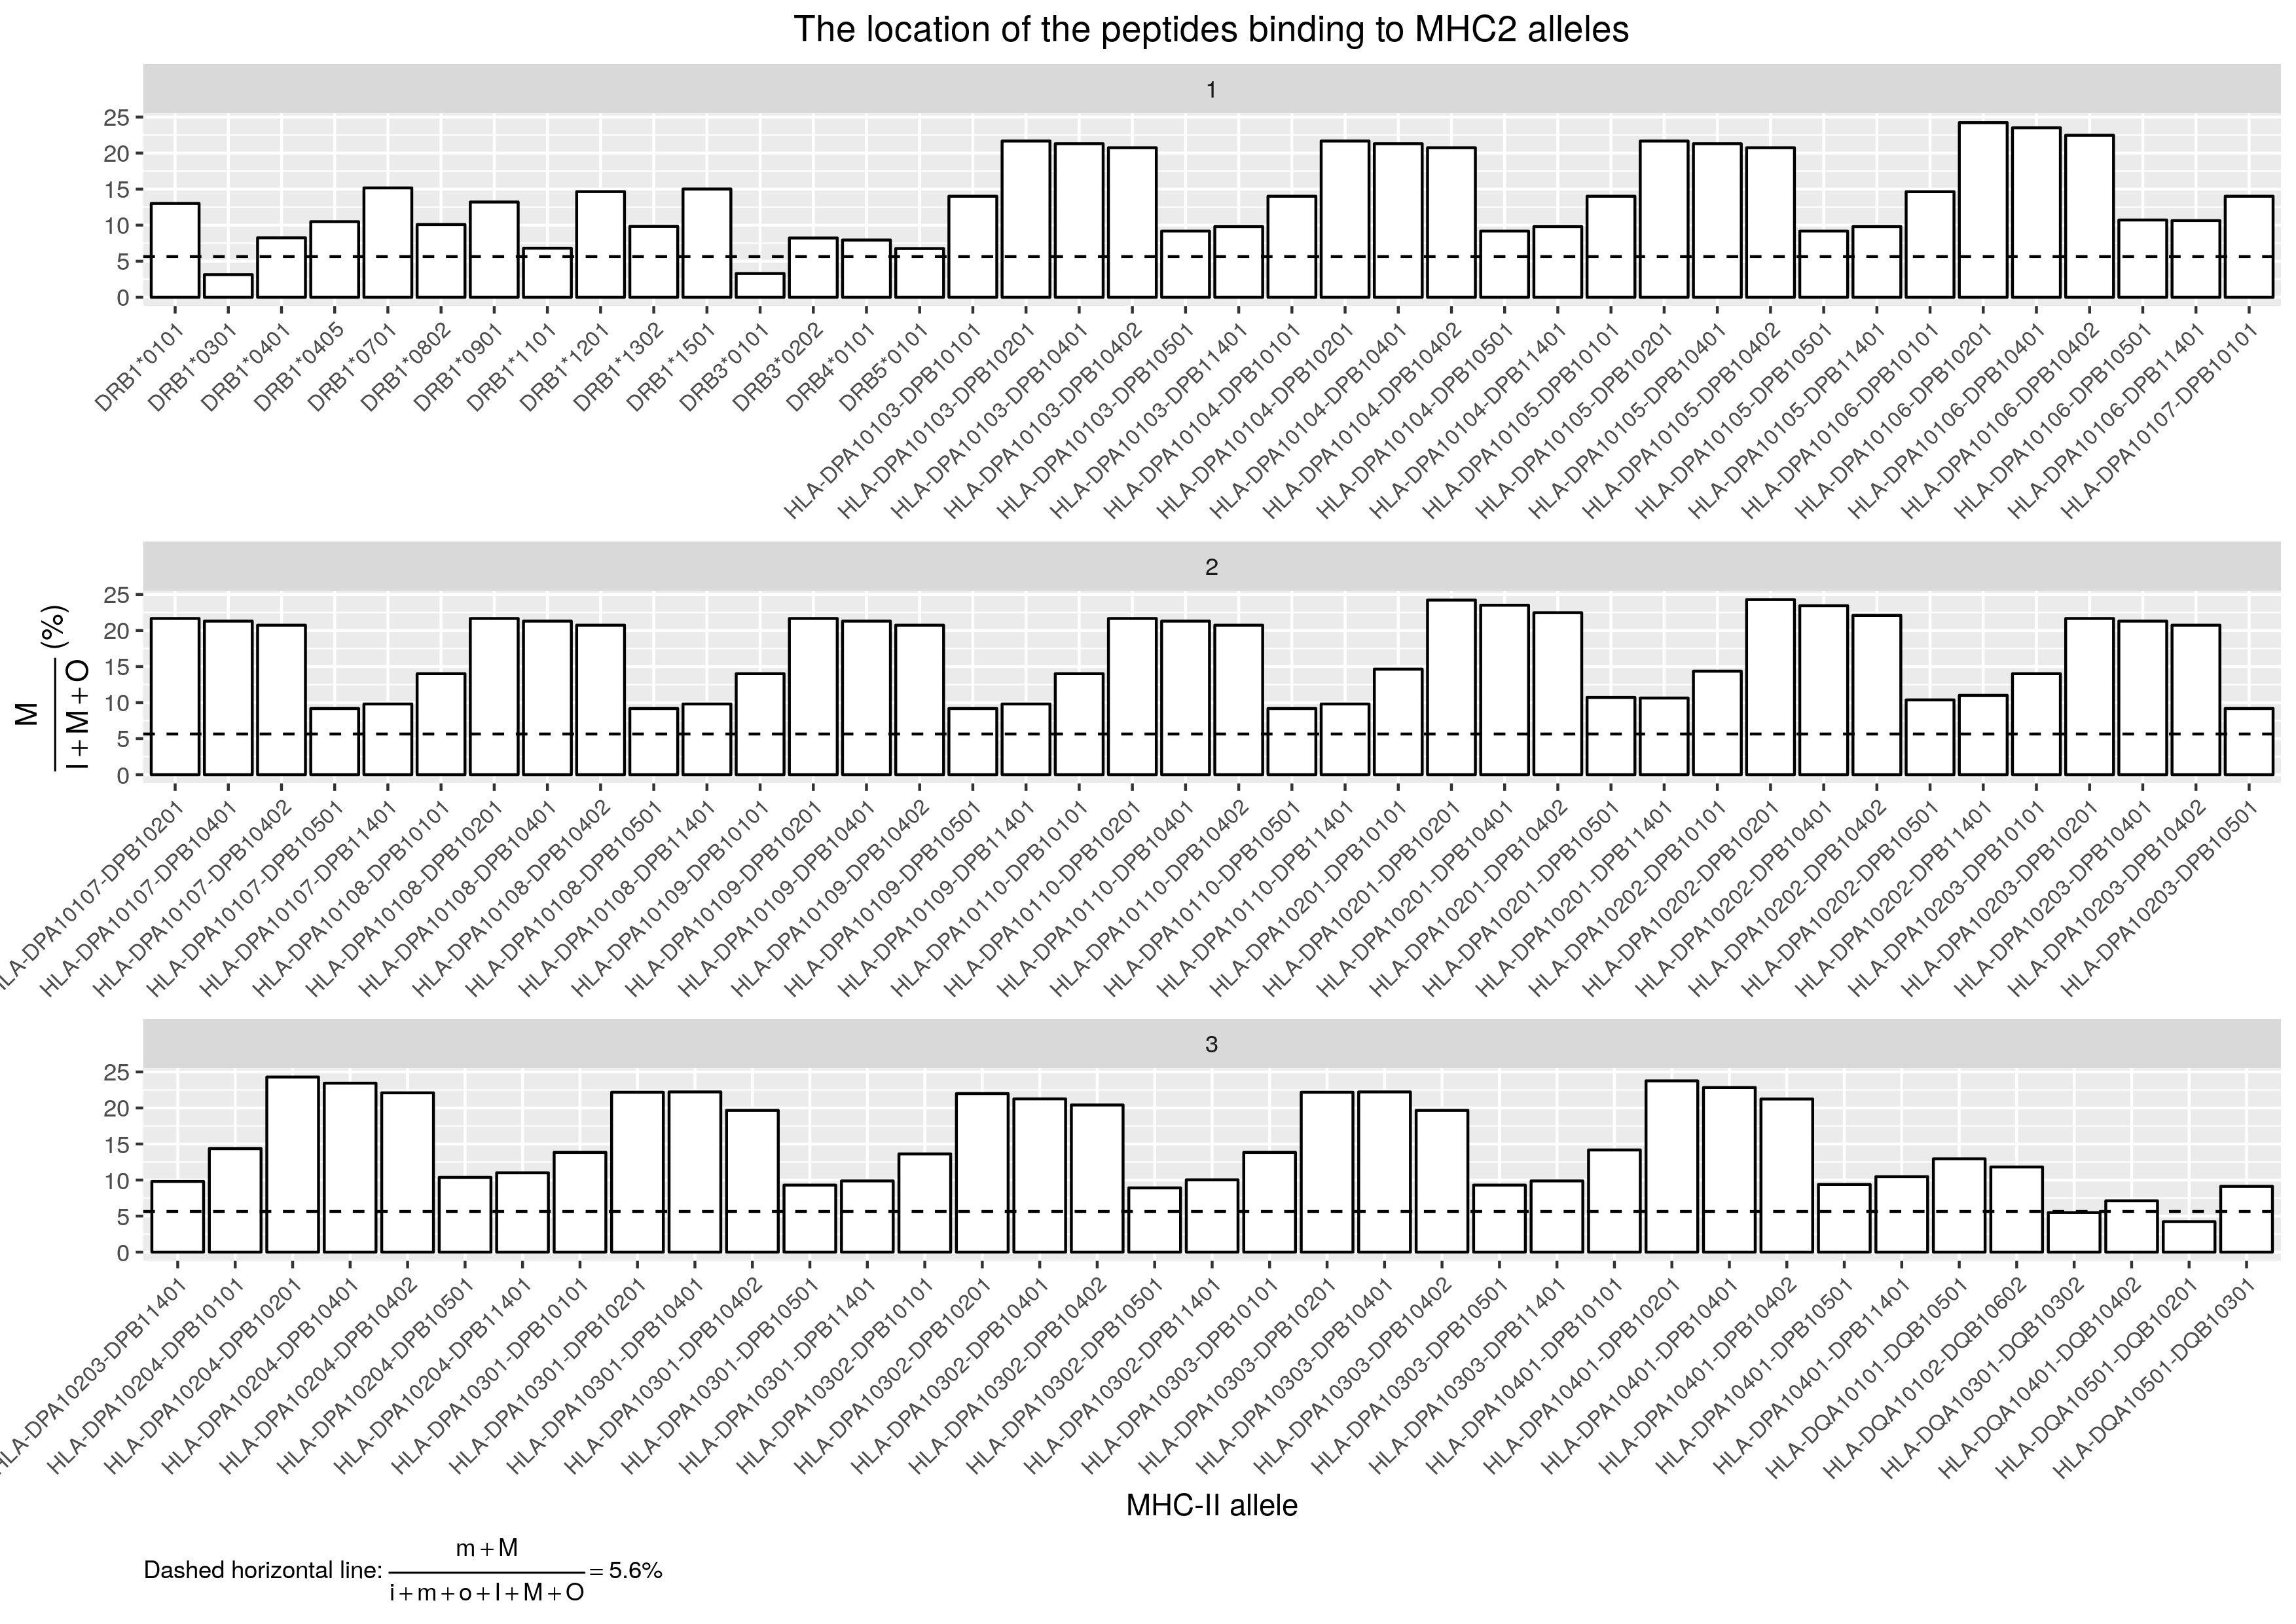
\includegraphics[width=\textwidth]{bbbq_3/figure_1.png}
	%   \label{fig:1}
	% \end{figure}

	% \begin{figure}[ht]
	%   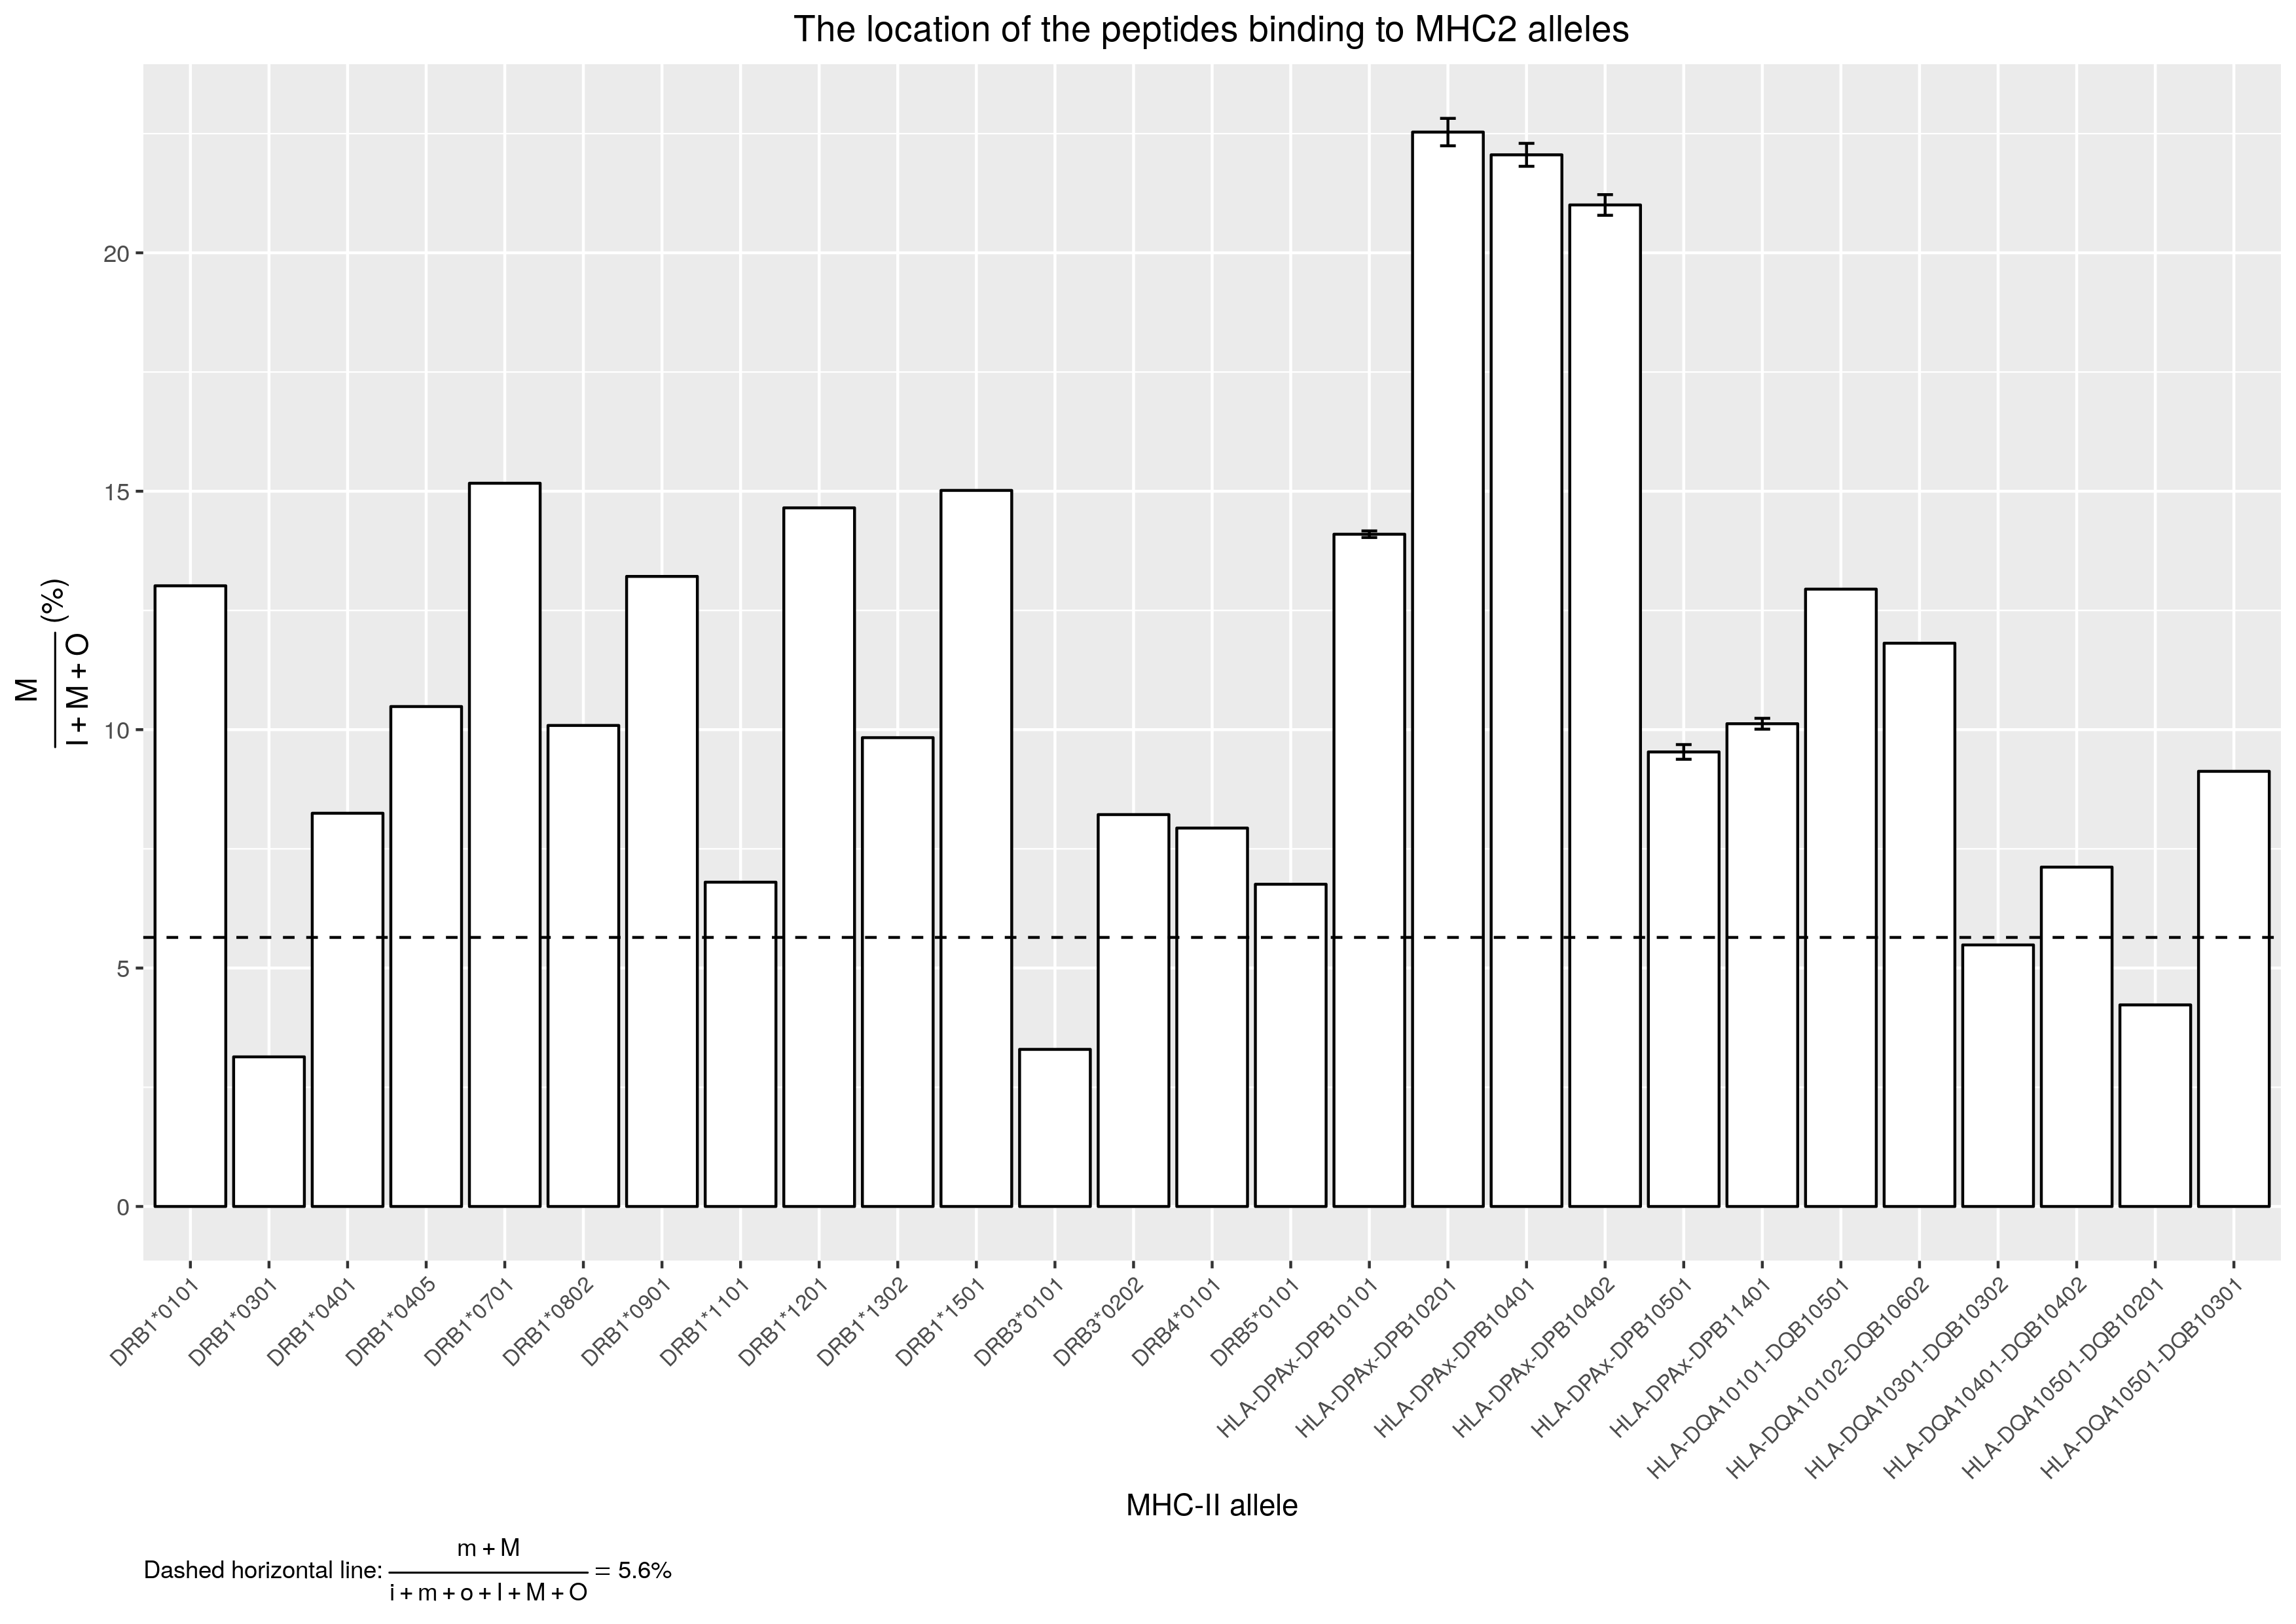
\includegraphics[width=\textwidth]{figure_1_5.png}
	%   \label{fig:1_5}
	% \end{figure}

	% \begin{figure}[ht]
	%   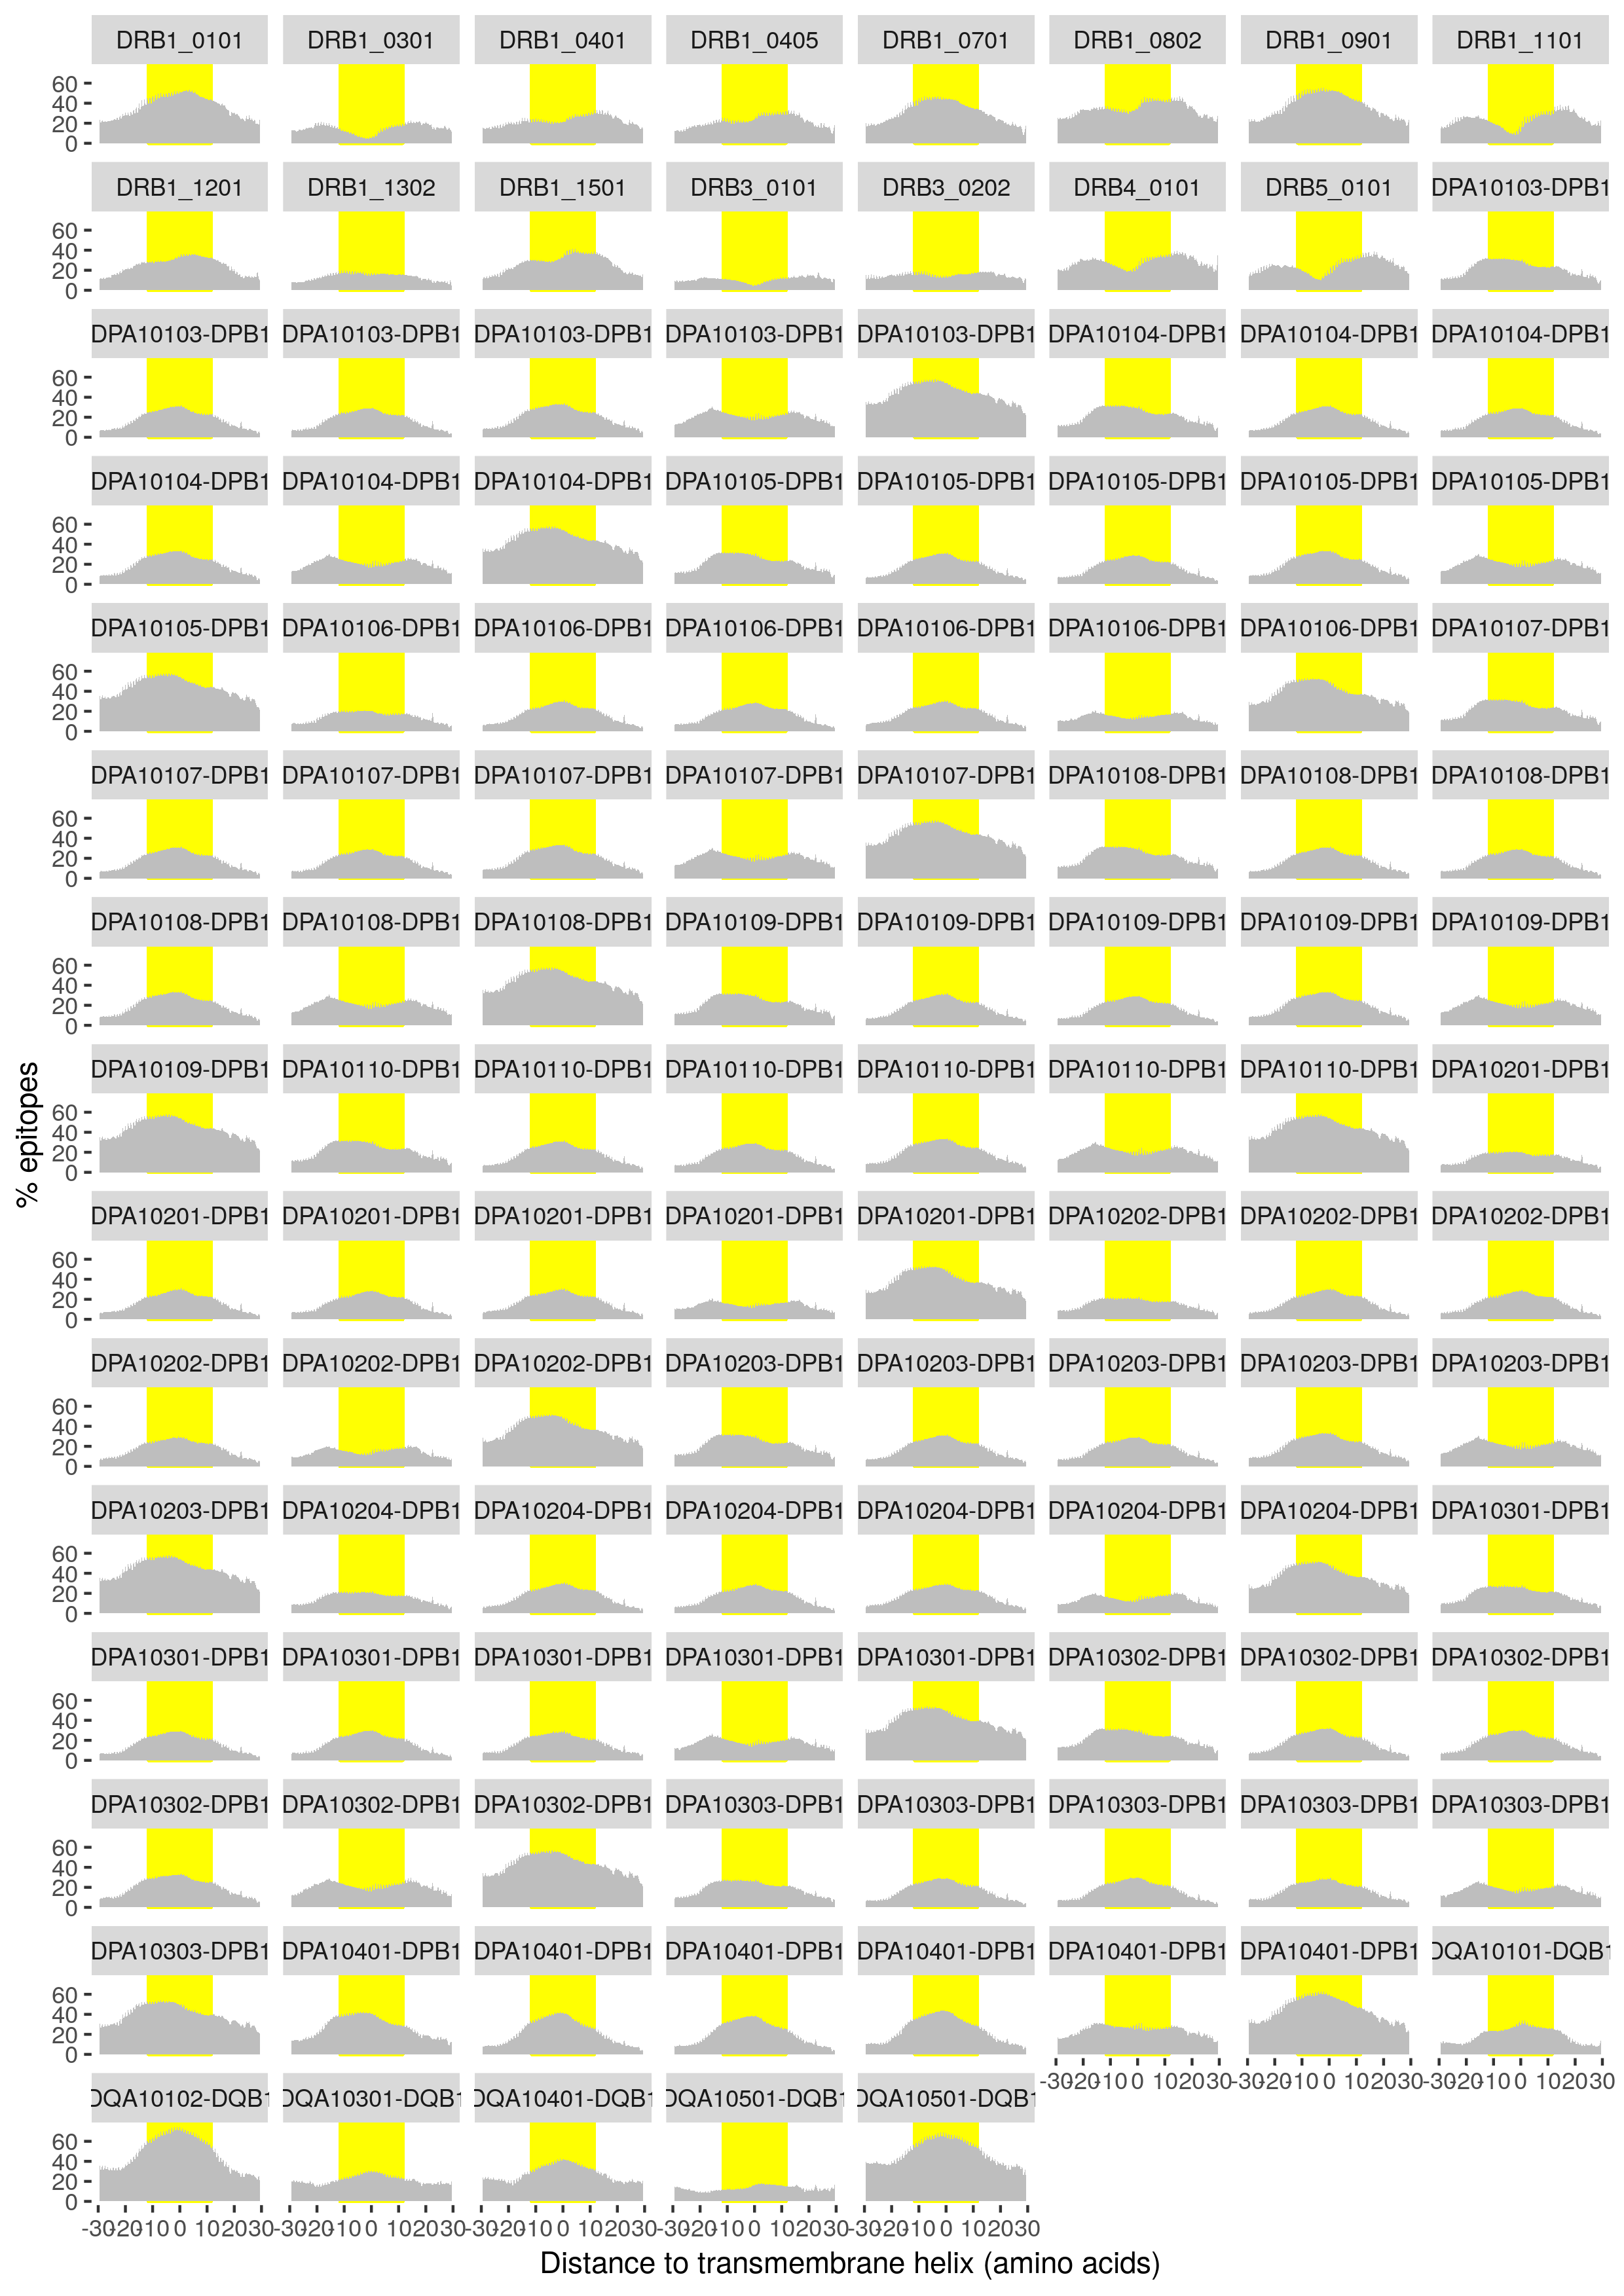
\includegraphics[width=\textwidth]{figure_3.png}
	%   \label{fig:3}
	% \end{figure}




	% \input{table_imoimo.latex}
	% % has label tab:results
	% \richel{
	%   I'd enjoy 
	%   (1) a row with 'expected by chance', 
	%   (2) using percentages instead,
	%   (3) merging inside and outside
	% }

	% The inference model with the highest evidence in the
	% TMH-only alignment was [yet unknown] and [also yet unknown]
	% for the non-TMH alignment. Individual model weights are shown
	% in tables \ref{tab:evidences_tmh} 
	% and \ref{tab:evidences_non_tmh}.

	% The Bayesian inference resulted in [a distribution of mutation rates],
	% as shown in [absent figure].
	% The ESSes of the Bayesian parameter estimates was above 200, exact values
	% are shown in tables \ref{tab:esses_tmh} and \ref{tab:esses_non_tmh}.

%%%%%%%%%%%%%%%%%%%%%%%%%%%%%%%%%%%%%%%%%%%%%%%%%%%%%%%%%%%%%%%%%%%%%%%%%%%%%%%%
\section{Conclusion}
%%%%%%%%%%%%%%%%%%%%%%%%%%%%%%%%%%%%%%%%%%%%%%%%%%%%%%%%%%%%%%%%%%%%%%%%%%%%%%%%

We found that the percentages of epitopes overlapping 
with TMHs for a human and COVID-19 proteome are 
[similar/different]. In other words, the
epitopes that MHC-I presents are [as/not as] likely 
to be derived from TMH within either a human host and its viral pathogen.

We found that the percentages of epitopes overlapping 
with TMHs for a human and Mycobacterium proteome are 
[similar/different]. In other words, the
epitopes that MHC-I presents are [as/not as] likely 
to be derived from TMH within either a human host and its bacterial pathogen.

	% We conclude that MHC-II binds to TMH peptides with a higher/lower/equal
	% probability than expected by chance. 

	% We conclude that the evolutionary conservation if the TMH parts of membrane
	% proteins is higher/less/equal compare to its non-TMH counterparts.

%%%%%%%%%%%%%%%%%%%%%%%%%%%%%%%%%%%%%%%%%%%%%%%%%%%%%%%%%%%%%%%%%%%%%%%%%%%%%%%%
\section{Discussion}
%%%%%%%%%%%%%%%%%%%%%%%%%%%%%%%%%%%%%%%%%%%%%%%%%%%%%%%%%%%%%%%%%%%%%%%%%%%%%%%%

We concluded that the
epitopes that MHC-I presents are [as/not as] likely 
to be derived from TMH within either a human host and its viral pathogen.
Because the full COVID-19 only has 4 TMHs \richel{check}, the percentages
of MHC-I epitopes being part of a TMH are likelier to be affected by
stochasticity. We chose to use COVID-19 regardless, as the thousands
of its time-dated genomic sequences are ideal for determining the 
evolutionary conservation of MHC-I detecting TMHs. 

We concluded that the
epitopes that MHC-I presents are [as/not as] likely 
to be derived from TMH within either a human host and its bacterial pathogen.
Because a bacterium does not infect a cell, thus its polypeptides
will not be presented by MHC-I, this result is [unexpected/expected]

	% \frans{
	%   De TMH evolutie data van COVID is missachien interresanter. Ik zie het als volgt. 
	%   COVID is een mooi voorbeeld van een virus 
	%   Myco van een bacterie
	%   In de bacterie is duidelijk dat tenmisnte voor MHCII TMHs zijn overgrepresenteerd virus niet. 
	%   Dus verhaal kan zijn dat TMHs belangrijk voot bacteirele afweer niet zozeer voor virussen. 
	% 
	%   Hiervoor moeten we MHC-I doen voor myco
	%   Kijken wat evolutie data doet voor virus dan evt kijken wat dit doet voor myco en vergelijken. 
	% }
	% 
	% We compared the mutation rates between the TMH and non-TMH part of
	% multiple mycobacterium species. Where we expect no variation 
	% in mutation rate for every TMH amino acid,
	% \richel{
	%   we can test this, but unsure if that would make sense
	% }
	% we know that non-TMH part will have regions of different evolutionary
	% conservation: functional domains, especially in protein-protein
	% interactions will be strongly conserved, due to an even more constrained
	% set of peptides that enable a certain function.

	% \richel{
	%   Note that most bacteria are opportunistic pathogens.
	%   Note that most bacteria are generalists.
	%   Note that most bacteria have different cell membranes (and walls), that
	%   may have different functional constraints than a human cell membrane
	% }

%%%%%%%%%%%%%%%%%%%%%%%%%%%%%%%%%%%%%%%%%%%%%%%%%%%%%%%%%%%%%%%%%%%%%%%%%%%%%%%%
\section{Acknowledgments}
%%%%%%%%%%%%%%%%%%%%%%%%%%%%%%%%%%%%%%%%%%%%%%%%%%%%%%%%%%%%%%%%%%%%%%%%%%%%%%%%

We thank the Center for Information Technology of the University 
of Groningen for its support and for providing access to the Peregrine 
high performance computing cluster. 

%%%%%%%%%%%%%%%%%%%%%%%%%%%%%%%%%%%%%%%%%%%%%%%%%%%%%%%%%%%%%%%%%%%%%%%%%%%%%%%%
\section{Data Accessibility}
%%%%%%%%%%%%%%%%%%%%%%%%%%%%%%%%%%%%%%%%%%%%%%%%%%%%%%%%%%%%%%%%%%%%%%%%%%%%%%%%

All code is archived at \url{http://github.com/richelbilderbeek/someplace},
with DOI \url{https://doi.org/12.3456/zenodo.1234567}.

%%%%%%%%%%%%%%%%%%%%%%%%%%%%%%%%%%%%%%%%%%%%%%%%%%%%%%%%%%%%%%%%%%%%%%%%%%%%%%%%
\section{Authors' contributions}
%%%%%%%%%%%%%%%%%%%%%%%%%%%%%%%%%%%%%%%%%%%%%%%%%%%%%%%%%%%%%%%%%%%%%%%%%%%%%%%%

RJCB and FB conceived the idea for this research. 
RJCB wrote the code.
RJCB and FB wrote the article.

%%%%%%%%%%%%%%%%%%%%%%%%%%%%%%%%%%%%%%%%%%%%%%%%%%%%%%%%%%%%%%%%%%%%%%%%%%%%%%%%
% Bibliography
%%%%%%%%%%%%%%%%%%%%%%%%%%%%%%%%%%%%%%%%%%%%%%%%%%%%%%%%%%%%%%%%%%%%%%%%%%%%%%%%
% MEE style
\bibliographystyle{mee}
\bibliography{article}
%%%%%%%%%%%%%%%%%%%%%%%%%%%%%%%%%%%%%%%%%%%%%%%%%%%%%%%%%%%%%%%%%%%%%%%%%%%%%%%%


%%%%%%%%%%%%%%%%%%%%%%%%%%%%%%%%%%%%%%%%%%%%%%%%%%%%%%%%%%%%%%%%%%%%%%%%%%%%%%%%
\appendix
\section{Supplementary materials}
%%%%%%%%%%%%%%%%%%%%%%%%%%%%%%%%%%%%%%%%%%%%%%%%%%%%%%%%%%%%%%%%%%%%%%%%%%%%%%%%

%%%%%%%%%%%%%%%%%%%%%%%%%%%%%%%%%%%%%%%%%%%%%%%%%%%%%%%%%%%%%%%%%%%%%%%%%%%%%%%%
\subsection{MHC-I}
%%%%%%%%%%%%%%%%%%%%%%%%%%%%%%%%%%%%%%%%%%%%%%%%%%%%%%%%%%%%%%%%%%%%%%%%%%%%%%%%

\begin{table}
  \input{bbbq_1/bbbq_1_percentages.latex}
  \caption{
    Percentage of MHC-I epitopes overlapping with transmembrane helix.
    \richel{This is simulated data}
  }
  \label{table:bbbq_1_percentages}
\end{table}

\begin{table}
  \input{bbbq_1/bbbq_1_stats_covid.latex}
  \caption{
    Kolmogorov-Smirnov test results comparing human and COVID-19 for MHC-I
    \richel{Done on the simulated data}
  }
  \label{table:bbbq_1_stats_covid}
\end{table}

\begin{table}
  \input{bbbq_1/bbbq_1_stats_myco.latex}
  \caption{
    Kolmogorov-Smirnov test results comparing human and Mycobacterium for MHC-I
    \richel{Done on the simulated data}
  }
  \label{table:bbbq_1_stats_myco}
\end{table}

%%%%%%%%%%%%%%%%%%%%%%%%%%%%%%%%%%%%%%%%%%%%%%%%%%%%%%%%%%%%%%%%%%%%%%%%%%%%%%%%
\subsection{MHC-II}
%%%%%%%%%%%%%%%%%%%%%%%%%%%%%%%%%%%%%%%%%%%%%%%%%%%%%%%%%%%%%%%%%%%%%%%%%%%%%%%%

\begin{table}
  \input{bbbq_2/bbbq_2_percentages.latex}
  \caption{
    Percentage of MHC-II epitopes overlapping with transmembrane helix.
    \richel{This is simulated data}
  }
  \label{table:bbbq_2_percentages}
\end{table}

\begin{table}
  \input{bbbq_2/bbbq_2_stats_covid.latex}
  \caption{
    Kolmogorov-Smirnov test results comparing human and COVID-19 for MHC-II
    \richel{Done on the simulated data}
  }
  \label{table:bbbq_2_stats_covid}
\end{table}

\begin{table}
  \input{bbbq_2/bbbq_2_stats_myco.latex}
  \caption{
    Kolmogorov-Smirnov test results comparing human and Mycobacterium for MHC-II
    \richel{Done on the simulated data}
  }
  \label{table:bbbq_2_stats_myco}
\end{table}

%%%%%%%%%%%%%%%%%%%%%%%%%%%%%%%%%%%%%%%%%%%%%%%%%%%%%%%%%%%%%%%%%%%%%%%%%%%%%%%%
\subsection{COVID-19 genome and proteome}
%%%%%%%%%%%%%%%%%%%%%%%%%%%%%%%%%%%%%%%%%%%%%%%%%%%%%%%%%%%%%%%%%%%%%%%%%%%%%%%%

\richel{
  This is just a reminder, instead of new research. 
  This subsection be deleted in the future.
}

\begin{figure}[!htbp]
  \includegraphics[width=0.9\textwidth]{pics/covid_genome_and_proteome.png}
  \caption{
    Overview of COVID-19 genome and proteome.
    From 
    \url{https://zhanglab.ccmb.med.umich.edu/COVID-19}
  }
  \label{fig:covid_genome_and_proteome}
\end{figure}

%%%%%%%%%%%%%%%%%%%%%%%%%%%%%%%%%%%%%%%%%%%%%%%%%%%%%%%%%%%%%%%%%%%%%%%%%%%%%%%%
\subsection{COVID-19 TMHs}
%%%%%%%%%%%%%%%%%%%%%%%%%%%%%%%%%%%%%%%%%%%%%%%%%%%%%%%%%%%%%%%%%%%%%%%%%%%%%%%%

\begin{figure}[!htbp]
  \includegraphics[width=\textwidth]{tmhs/tmhs.png}
  \caption{
    Location of amino acids of reference COVID-19 proteome.
    Note that ORF1a results in multiple proteins, 
    as shown in figure \ref{fig:covid_genome_and_proteome}.
    Legend: i = inside (cytosolic side), m = membrane, o = outside (extracellular side)
    \richel{This is real data}
  }
  \label{fig:covid_locatome}
\end{figure}


%%%%%%%%%%%%%%%%%%%%%%%%%%%%%%%%%%%%%%%%%%%%%%%%%%%%%%%%%%%%%%%%%%%%%%%%%%%%%%%%
\subsection{MHC-II haplotype occurrences}
%%%%%%%%%%%%%%%%%%%%%%%%%%%%%%%%%%%%%%%%%%%%%%%%%%%%%%%%%%%%%%%%%%%%%%%%%%%%%%%%

\richel{
  This is just a reminder, instead of new research. 
  This subsection be deleted in the future.
}

\begin{table}
  \input{mhc2_haplotypes.latex}
  \caption{
    Percentage of MHC-II haplotypes, from \cite{greenbaum2011functional}
    \richel{
      This is just a reminder, instead of new research. 
      This table be deleted in the future.
    }
  }
  \label{table:mhc2_haplotypes}
\end{table}

%%%%%%%%%%%%%%%%%%%%%%%%%%%%%%%%%%%%%%%%%%%%%%%%%%%%%%%%%%%%%%%%%%%%%%%%%%%%%%%%
\subsection{Kolmogorov-Smirnov}
%%%%%%%%%%%%%%%%%%%%%%%%%%%%%%%%%%%%%%%%%%%%%%%%%%%%%%%%%%%%%%%%%%%%%%%%%%%%%%%%

\richel{
  This is just a reminder, instead of new research. 
  This subsection be deleted in the future.
}

The Kolmogorov-Smirnov (KS) test determines if two samples
are derived from the same distribution, without making assumptions
regarding the shape of that distribution. 

We will reject
the null hypothesis that MHC-I has the same percentage of epitopes 
overlapping with TMHs in Homo sapiens compared to each pathogen when 
the KS statistic $D_{n,m}$ follows the relationship as shown in 
equation \ref{eq:ks}, for a significance level $\alpha = 0.05$
and $n = m$ equals the number of HLA haplotypes.

\begin{equation}
   D_{n,m} > \frac{1}{\sqrt{n}} \cdot \sqrt{ -\ln(\frac{\alpha}{2}) \cdot \frac{1 + \frac{n}{m}}{2} }
   \label{eq:ks}
\end{equation}

\end{document}
new research. 
      This table be deleted in the future.
    }
  }
  \label{table:mhc2_haplotypes}
\end{table}

%%%%%%%%%%%%%%%%%%%%%%%%%%%%%%%%%%%%%%%%%%%%%%%%%%%%%%%%%%%%%%%%%%%%%%%%%%%%%%%%
\subsection{Kolmogorov-Smirnov}
%%%%%%%%%%%%%%%%%%%%%%%%%%%%%%%%%%%%%%%%%%%%%%%%%%%%%%%%%%%%%%%%%%%%%%%%%%%%%%%%

\richel{
  This is just a reminder, instead of new research. 
  This subsection be deleted in the future.
}

The Kolmogorov-Smirnov (KS) test determines if two samples
are derived from the same distribution, without making assumptions
regarding the shape of that distribution. 

We will reject
the null hypothesis that MHC-I has the same percentage of epitopes 
overlapping with TMHs in Homo sapiens compared to each pathogen when 
the KS statistic $D_{n,m}$ follows the relationship as shown in 
equation \ref{eq:ks}, for a significance level $\alpha = 0.05$
and $n = m$ equals the number of HLA haplotypes.

\begin{equation}
   D_{n,m} > \frac{1}{\sqrt{n}} \cdot \sqrt{ -\ln(\frac{\alpha}{2}) \cdot \frac{1 + \frac{n}{m}}{2} }
   \label{eq:ks}
\end{equation}

\end{document}
